\RequirePackage[OT1]{fontenc} 
\documentclass[journal]{IEEEtran}

% *** CITATION PACKAGES ***
\usepackage[style=ieee]{biblatex} 
\bibliography{example_bib.bib}    %your file created using JabRef

% *** MATH PACKAGES ***
\usepackage{amsmath}
\usepackage{amssymb}

% Table Packages
\usepackage{booktabs}
\usepackage{tabularx}

% *** PDF, URL AND HYPERLINK PACKAGES ***
\usepackage{url}
% correct bad hyphenation here
\hyphenation{op-tical net-works semi-conduc-tor}
\usepackage{graphicx}  %needed to include png, eps figures
\graphicspath{{./images/}}
\usepackage{float}  % used to fix location of images i.e.\begin{figure}[H]

%Mathcha
\usepackage{physics}
\usepackage{amsmath}
\usepackage{tikz}
\usepackage{mathdots}
\usepackage{yhmath}
\usepackage{cancel}
\usepackage{color}
\usepackage{siunitx}
\usepackage{array}
\usepackage{multirow}
\usepackage{amssymb}
\usepackage{gensymb}
\usepackage{tabularx}
\usepackage{extarrows}
\usepackage{booktabs}
\usetikzlibrary{fadings}
\usetikzlibrary{patterns}
\usetikzlibrary{shadows.blur}
\usetikzlibrary{shapes}

\newcommand{\eqdef}{\mathrel{:\mathop=}}

\begin{document}

\title{Stereo Radio Signals}
% \\ \small{EE4361 Class Project}

% author names 
\author{STEPHEN ANSEL CAMPBELL \\
    \emph{sac170630@utdallas.edu} \\
    EE 4361 --- INTRO TO DIGITAL SIGNAL PROCESSING
}

% The report headers
\markboth{EE 4361 Dr. Issa Panahi, \today}%do not delete next lines
{EE 4361 Dr. Panahi}

% make the title area
\maketitle

% As a general rule, do not put math, special symbols or citations
% in the abstract or keywords.
\begin{abstract}
    Overall, In this lab  overall familiarity with the key parameters and
    performance of practical RF mixer was gained. The importance of Conversion Loss
    was shown to be of tantamount significance. The non idealities of mixer's was
    evident through these precise lab measurements.
\end{abstract}

\section{Introduction}

\IEEEPARstart{T}{his} lab utilizes the spectrum analyzer, signal generator, and VNA acting as a
signal generator to determine the conversion loss of the mixer under test. The
VNA is also used to characterize the Mixer's Return Loss. An important aspect of
this lab entails accounting for the cable loss present between the signal
generator and the mixer LO. This Loss is calculated given the direct measurement
with the spectrum analyzer.

\section{Formulation}

\textbf{Develop and write down the complete analytical formulation of the
    problem, at the transmitter and at the receiver and, how and why \(x_1(n)\) and
    \(x_2(n)\)and the gains are obtained in your report.}

Starting as analog signals
\begin{gather*}
    \text{Time Domain}\\
    \begin{aligned}
        x_{1,a}( t) & \eqdef \text{male speaker}   \\
        x_{2,a}( t) & \eqdef \text{female speaker}
    \end{aligned}
\end{gather*}


Bandlimited to 5kHz through low pass filtering


\begin{equation*}
    \begin{aligned}
        x_{1,\text{bandlimited}}( t) & =x_{1,a}( t) *h_{lp,f_{c} =5\text{kHz}}( t) \\
        x_{2,\text{bandlimited}}( t) & =x_{2,a}( t) *h_{lp,f_{c} =5\text{kHz}}( t)
    \end{aligned}
\end{equation*}


Sampling at 16kHz more than double the bandlimited, \(\displaystyle
F_{s,\text{mic}} =16\times 10^{3}\text{Hz} ,\ T_{s,\text{mic}}
=1/F_{s,\text{mic}}\) and windowing between 0 and \(\displaystyle T_{F}\)

\begin{equation*}
    \begin{aligned}
        x_{1}( n) & =x_{1,\text{bandlimited}}( t)\Bigr|_{t=nT_{s,\text{mic}}} ,\ 0< nT_{s,\text{mic}} < T_{F}    \\
        x_{2}( n) & =x_{2,\text{bandlimited}}( t) \ \Bigr|_{t=nT_{s,\text{mic}}} ,\ 0< nT_{s,\text{mic}} < T_{F}
    \end{aligned}
\end{equation*}


Addition and Subtraction
\begin{equation*}
    \begin{aligned}
        s_{1}( n) & =x_{1}( n) +x_{2}( n) \\
        s_{2}( n) & =x_{1}( n) -x_{2}( n)
    \end{aligned}
\end{equation*}


Modulation at $\displaystyle f_{\text{carrier}} =70\text{kHz}$ and \ $\displaystyle f_{\text{carrier}} +f_{\Delta } =90\text{kHz}$
\begin{align*}
    \begin{aligned}
        s_{1,\text{modulated}}( n) & =s_{1}( n)\cos\left(\frac{2\pi f_{\text{carrier}}}{F_{s,\text{mic}}} n\right)                 \\
        s_{2,\text{modulated}}( n) & =s_{2}( n)\cos\left(\frac{2\pi ( f_{\text{carrier}} +f_{\Delta })}{F_{s,\text{mic}}} n\right)
    \end{aligned} &  & \begin{aligned}
                            & \\
                            &
                       \end{aligned}
\end{align*}
Addition and Subtraction
\begin{align*}
    \begin{aligned}
        TX( n) & =s_{1,\text{modulated}}( n) +s_{2,\text{modulated}}( n)
    \end{aligned} &  & \begin{aligned}
                            & \\
                            &
                       \end{aligned}
\end{align*}
D/A
\begin{equation*}
    \begin{aligned}
        TX( t) & =\sum _{k=-\infty }^{\infty } TX( k) \delta ( t+kT_{s}) *h_{lp,f_{c} =90\text{kHz}}( t)
    \end{aligned}
\end{equation*}
Lossless Transmission


\begin{align*}
    RX( t) & =TX( t)
\end{align*}


A/D with sampling freqency and sample interval $\displaystyle F_{s,\text{receiver}} =400\times 10^{3}\text{Hz} ,\ T_{s,\text{receiver}} =1/F_{s,\text{receiver}}$ and windowing between 0 and $\displaystyle T_{F}$


\begin{align*}
    RX( n) & =RX( t)\Bigr|_{t=nT_{s,\text{receiver}}} ,\ 0< nT_{s,\text{receiver}} < T_{F} \
\end{align*}
Black Box Receiver


\begin{align*}
    \operatorname{RECV}                  & \eqdef \text{Receiver to be designed}        \\
    \tilde{x}_{1}( n) ,\tilde{x}_{2}( n) & =\operatorname{RECV}_{1}\left( RX( n)\right)
\end{align*}





\section{Design}
the $\displaystyle \operatorname{RECV}$ operation is given as the below signal processing pipeline.



Demodulation
\begin{align*}
    RX_{\text{demodulated, 70kHz}}( n) & =RX( n)\cos\left(\frac{2\pi f_{\text{carrier}}}{F_{s,\text{receiver}}} n\right)                 \\
    RX_{\text{demodulated, 90kHz}}( n) & =RX( t)\cos\left(\frac{2\pi ( f_{\text{carrier}} +f_{\Delta })}{F_{s,\text{receiver}}} n\right)
\end{align*}
Filtering
\begin{align*}
    s_{1}( n) & =RX_{\text{demodulated, 70kHz}}( n) *h_{lp,f_{c} =5\text{kHz}}( n) \\
    s_{2}( n) & =RX_{\text{demodulated, 90kHz}}( n) *h_{lp,f_{c} =5\text{kHz}}( n)
\end{align*}


Addition and Subtraction


\begin{align*}
    \tilde{x}_{1}( n) & =G_{1}\left( s_{1}( n) +s_{2}( n)\right) \\
    \tilde{x}_{2}( n) & =G_{2}\left( s_{1}( n) -s_{2}( n)\right) \\
    G_{1} ,G_{2}      & \rightarrow \frac{1}{2}
\end{align*}
\section{Results}
\begin{figure}
    \begin{center}
        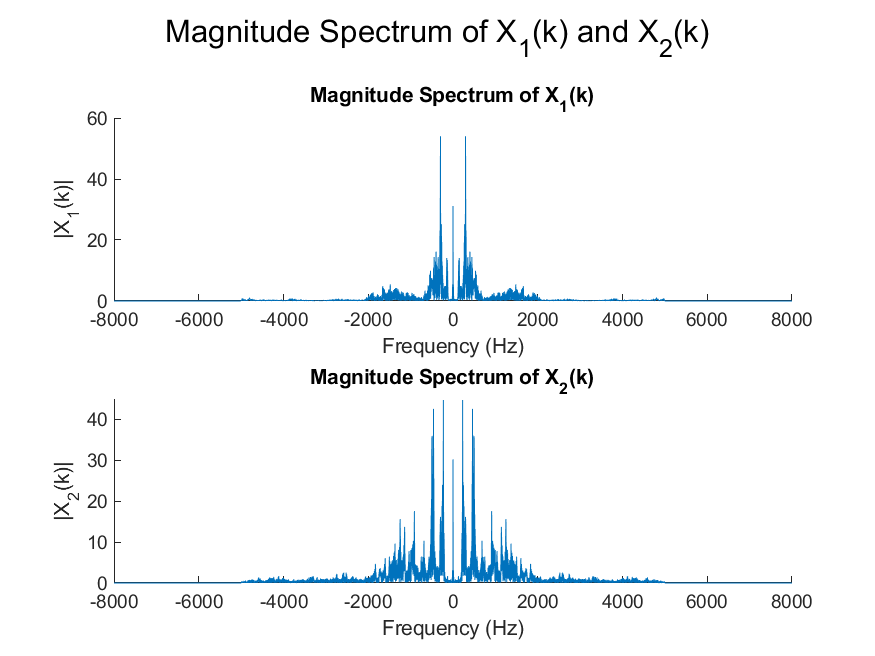
\includegraphics[width=0.4\textwidth]{freq_recon.png}
        \caption{\label{fig:freq_recon}Magnitude of DFT of Reconstructed Signals \(x_1(n)\) and \(x_2(n)\)}
    \end{center}
\end{figure}

\begin{figure}
    \begin{center}
        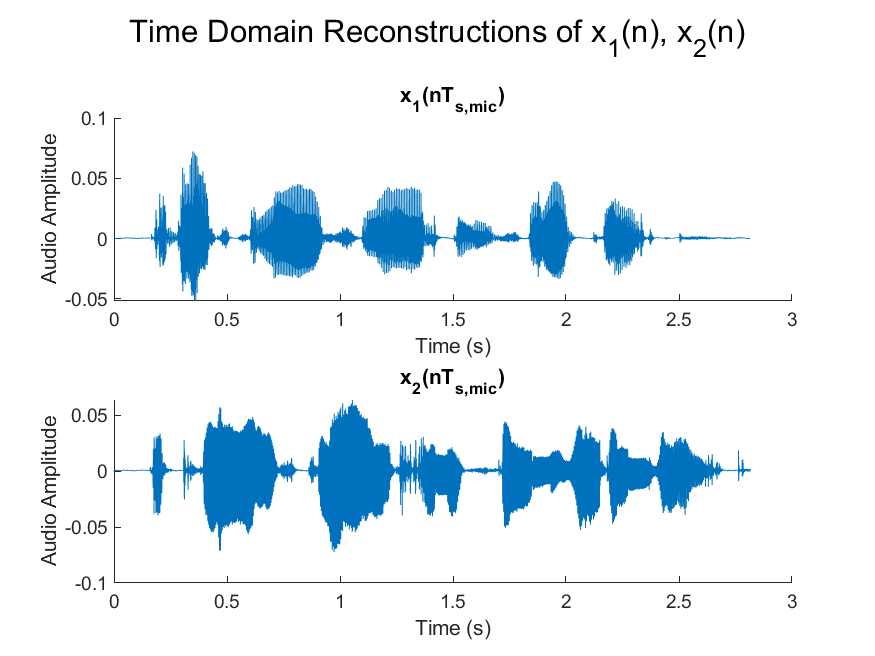
\includegraphics[width=0.4\textwidth]{time_recon.png}
        \caption{\label{fig:time_recon} Time Domain Representation of Reconstructed Signals \(x_1(n)\) and \(x_2(n)\)}
    \end{center}
\end{figure}

% \appendices
% \section{Pre-Lab}
% \section{Extra Photos}

\end{document}